\documentclass[../main.tex]{subfiles}

\begin{document}
    \subsection{パイプライン処理}
    本プロセッサでは、逐次実行で実装するのあれば、かなりのクロック数を無駄にするため、
    複数の命令を同時に並列的に実行するためには
    5段パイプライン処理を導入し、それらの5ステージの詳細は以下のように構成される。

    \begin{itemize}
        \item IF ステージ \\
            取得する命令アドレスを計算し,命令メモリから次々と実行すべき命令をフェッチする。
        \item ID ステージ \\
            フェッチされた命令をデコードし,必要とする制御信号を解釈する。
            また、デコードされた命令種類に対し、即値の拡張を行う。
            ここで、ストール検出「詳細は\ref{sssec:stall}」とデータ依存検出「詳細は\ref{ssec:hazard}」も行う。
        \item EX ステージ \\
            命令の種類から,行うべき演算を実行する
            ここで、IDステージで解釈された命令の種類が分岐命令であり、分岐条件が満たしていれば、
            分岐先のアドレスも計算する「詳細は\ref{ssec:aluImprove}」。
        \item MEM ステージ \\
           主にロード命令またはストア命令を扱うステージである。
           メモリアドレスを指定し,データメモリからデータをロードもしくはデータをストアする。
           ただし、ロードされたデータを命令の種類により拡張する。
        \item WB ステージ \\
            レジスタへの書き込みを行う。
    \end{itemize}

    \subsection{データハザードとその解決方法} \label{ssec:hazard}
        本プロセッサは5段パイプラインで実装されているため、いくつかの問題が発生する。
        パイプライン化をすることで、EXステージで実行している命令と以前に実行していた命令にデータの依存関係があり得る。
        つまり、データハザードが生じ、逐次に実行したときとの最終結果が変わり、結果の保証ができなくなる。
        本プロセッサでは、ハザードは主に2つの場合があり、LOAD命令の場合とLOAD命令でない場合である。
        詳細は、\ref{sssec:forwarding}にある。
        ハザード検出の原理は、3つのパイプライン、IF/IDパイプライン、ID/EXパイプライン、EX/MEMパイプラインを基に検出する。
        それぞれのパイプラインには現在各ステージで実行している命令を格納しているため、
        その命令から関係するレジスタを取り出し、検出を行う。
        従って、パイプラインストールおよびデータフォワーディングという概念を導入する必要がある。
        ここで、注意すべきところは、
        ハザード検出には2つ同様なユニットからできているため、
        書き込みのレジスタは重なる可能性がある。
        よって、場合分けする必要があり、そのどれかを1つしか選べない状態にする。

        \begin{figure}[h]
            \centering
            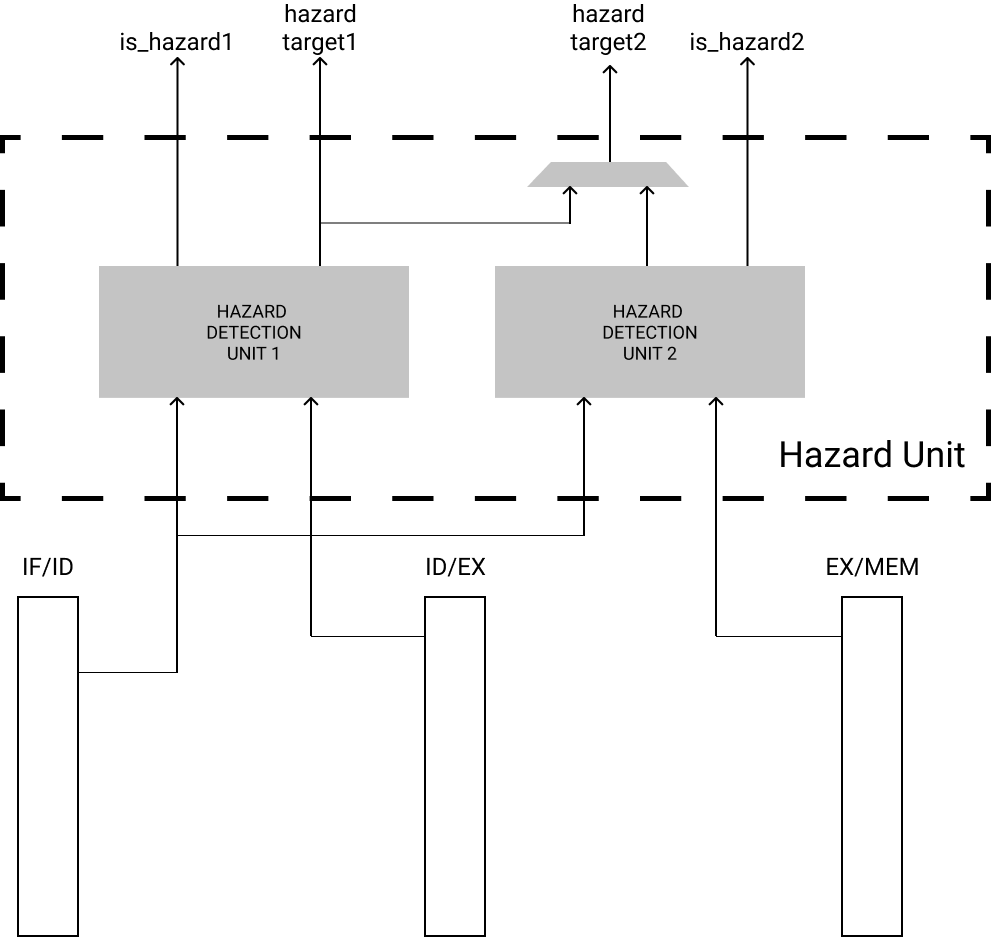
\includegraphics[width = 1.2\columnwidth]{../images/hazard.png}
            \caption{データフォワーディング}
            \label{fig:forwarding}
        \end{figure}
        
        \subsubsection{データフォワーディング} \label{sssec:forwarding}
        フォワーディングとは、EXステージでの命令と前の命令にハザードが生じたときに、
        前命令のEXステージからの計算結果をEXステージにフォワードする。
        ただし、LOAD命令にはEXステージではなく、
        MEMステージでデータメモリから取り出した値をEXステージで実行している命令にフォワードすること注意すべきである。
        本プロセッサで実装したデータフォワーディングは図\ref{fig:forwarding}に示す。

        \begin{figure}[h]
            \centering
            
\includegraphics[width = 1.2\columnwidth]{../images/forwarding.png}
            \caption{データフォワーディング}
            \label{fig:forwarding}
        \end{figure}

        \subsubsection{パイプラインストール} \label{sssec:stall}
            パイプラインストールが必要になった理由は、
            フォワーディングだけでは解決できないハザードに対抗するためである。
            例えば、EXステージでの命令は前の命令にデータ依存があり、
            前の命令がLOAD命令であるとき、
            EXステージではなく、MEMステージからのフォワーディングになる。
            つまり、1段を空けないといけない状態になっている。
            本プロセッサで実装したストールは図\ref{fig:stall}に示す。
            ストール信号を受けるIFステージは現在のPCの値に対し、4を引き、
            前の命令をフェッチすることになる。
            IF/IDパイプラインでは、その信号を受けると、プロセッサの状態を影響するような信号をゼロの信号を出力する。
            ただし、レジスタファイルに対する書き込みは負論理の信号なので、
            1の信号を出力ことになる。

            ただし、こうのような方法では1つの問題があり、
            その解決方法も含め、\ref{ssec:stallImprove}に詳しく述べる。

            \begin{figure}[h]
                \centering
                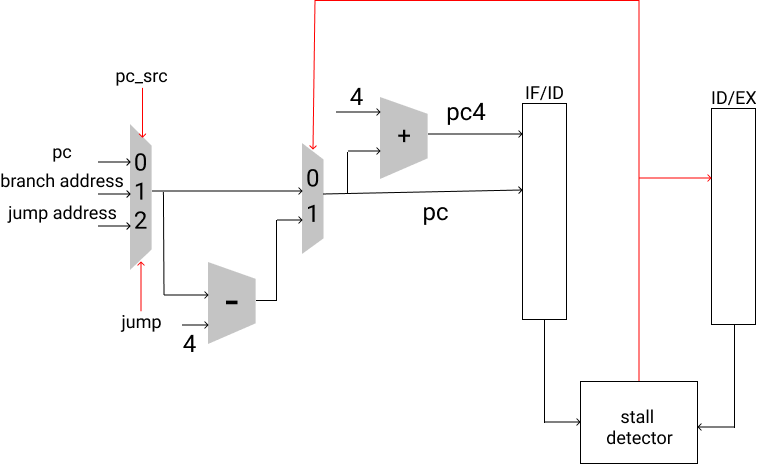
\includegraphics[width = 1.5\columnwidth]{../images/stall.png}
                \caption{パイプラインストール}
                \label{fig:stall}
            \end{figure}

    \subsection{制御ハザードその解決方法}
        ここでのプロセッサではを考え、
        制御ハザードとは分岐命令またはジャンプ命令にしか起こらないハザードである。
        ジャンプ命令はIDステージでわかるため、次から実行する命令はすでにフェッチされているため、
        ジャンプした後も、その命令はIDステージで実行することになる。
        よって、実行結果に影響を及ばさないためには、パイプラインフラッシュという概念を導入する。

    \subsubsection{パイプラインフラッシュ}
        パイプラインフラッシュとは、
        ジャンプまたは分岐の制御信号がアクティブであれば、
        パイプラインのある値にゼロまたは、意味をなさい信号(プロセッサに変化を持たさない信号)に書き換えるようにする。
        最低限、その命令を実行してもプロセッサの状態(レジスタおよびメモリへの書き込み)が変化しなければ良い。

\end{document}
